\documentclass[12pt]{article}
\usepackage{geometry}
\geometry{a4paper, portrait, margin=1in}

% --- Math Packages ---
\usepackage{amsmath}
\usepackage{amssymb}
\usepackage{amsfonts}
\usepackage{amsthm}

% --- Graphics & Diagrams ---
\usepackage{graphicx}
\usepackage{tikz}
\usetikzlibrary{shapes, arrows, positioning}

% --- Formatting ---
\usepackage{parskip}
\usepackage[hidelinks]{hyperref}
\usepackage{natbib}
\usepackage{enumitem}
\pagestyle{plain}

\title{HT Week 8 Model}
\author{Mohammad-Shah Karim}
\date{March 2026}

\begin{document}

\maketitle

\tableofcontents

\newpage

\section{Introduction}

This document outlines a game-theoretical model for pharmaceutical innovation and pricing to explain the empirical puzzle observed in the patent market following the expansion of Medicaid under the Affordable Care Act. The model captures the stochastic nature of R\&D, the specific procurement mechanism (PDL bidding) used by state agencies, and how current procurement outcomes dictate future innovation incentives.

Figure \ref{fig:game_structure} summarises the sequence of play, mapping the innovation decision in Period 1 to the pricing outcomes, which subsequently define the firm's state for future investment decisions in Period 2.

\begin{figure}[h]
    \centering
    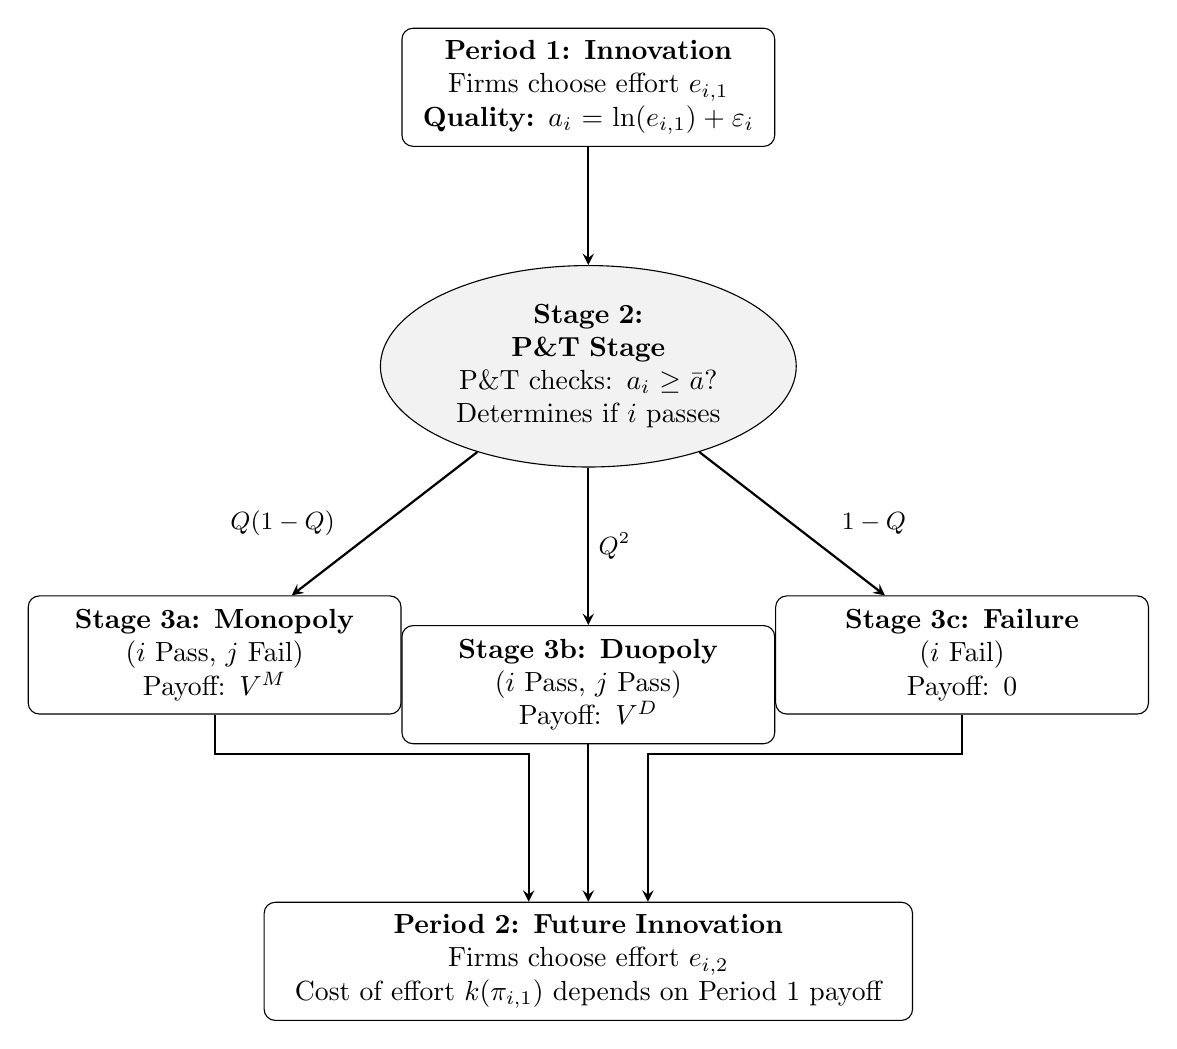
\begin{tikzpicture}[
        node distance=1.5cm and 1cm,
        auto,
        block/.style={rectangle, draw, fill=white, text width=4.5cm, align=center, rounded corners, minimum height=1.5cm},
        wideblock/.style={rectangle, draw, fill=white, text width=8cm, align=center, rounded corners, minimum height=1.5cm},
        cloud/.style={ellipse, draw, fill=gray!10, text width=3.5cm, align=center, minimum height=1.2cm},
        arrow/.style={thick,->,>=stealth}
    ]

    % Stage 1: Innovation
    \node [block] (stage1) {\textbf{Period 1: Innovation}\\ Firms choose effort $e_{i,1}$\\ \textbf{Quality:} $a_i = \ln(e_{i,1}) + \varepsilon_i$};

    % Stage 2: P&T Stage
    \node [cloud, below=of stage1] (pt) {\textbf{Stage 2: P\&T Stage}\\ P\&T checks: $a_i \ge \bar{a}$?\\ Determines if $i$ passes};
    
    % Stage 3: Pricing & Costs
    % Monopoly
    \node [block, below left=2cm and 0.5cm of pt] (mono) {\textbf{Stage 3a: Monopoly}\\ ($i$ Pass, $j$ Fail)\\ Payoff: $V^M$};
    
    % Duopoly
    \node [block, below=2cm of pt] (duo) {\textbf{Stage 3b: Duopoly}\\ ($i$ Pass, $j$ Pass)\\ Payoff: $V^D$};
    
    % Failure
    \node [block, below right=2cm and 0.5cm of pt] (fail) {\textbf{Stage 3c: Failure}\\ ($i$ Fail)\\ Payoff: $0$};

    % Period 2: Future Innovation
    \node [wideblock, below=2cm of duo] (period2) {\textbf{Period 2: Future Innovation}\\ Firms choose effort $e_{i,2}$ \\ Cost of effort $k(\pi_{i,1})$ depends on Period 1 payoff};

    % Connecting Lines
    \draw [arrow] (stage1) -- (pt);
    \draw [arrow] (pt) -- node[left, xshift=-0.5cm, font=\small] {$Q(1-Q)$} (mono);
    \draw [arrow] (pt) -- node[font=\small] {$Q^2$} (duo);
    \draw [arrow] (pt) -- node[right, xshift=0.5cm, font=\small] {$1-Q$} (fail);
    
    % Connections to Period 2
    \draw [arrow] (mono.south) -- ++(0,-0.5) -| (period2.135);
    \draw [arrow] (duo.south) -- (period2.north);
    \draw [arrow] (fail.south) -- ++(0,-0.5) -| (period2.45);

    \end{tikzpicture}
    \caption{The Sequence of Play: Innovation, P\&T Approval, Pricing, and Future Investment}
    \label{fig:game_structure}
\end{figure}

\newpage

\section{Stage 1: The Innovation Decision (Effort)}

First, firms make investment decisions for a drug they wish to market. Innovation is modelled to require effort - this is costly but improves the probability of clinical success.

\subsection{The Production Technology}
The realised clinical quality $a_i$ is a function of the effort exerted by the firm and a stochastic component $\varepsilon_i$:
\begin{equation}
    a_i = \ln(e_i) + \varepsilon_i, \qquad \varepsilon_i \sim N(0, \sigma^2)
\end{equation}
where $\varepsilon_i$ represents the inherent uncertainty of the R\&D process.

\subsection{The Cost of Effort}
Firms $i$ and $j$ simultaneously choose R\&D effort levels $e_i \geq 0$. Effort is assumed to be costly and convex:
\begin{equation}
    C(e_i) = \frac{1}{2} k e_i^2
\end{equation}

\newpage

\section{Stage 2: The P\&T Stage}
Once effort is exerted it is now a sunk cost, nature determines the clinical outcome of each firm's drug $a_i$, i.e. whether the drug passes the P\&T stage.

\subsection{The Approval Condition}
A drug is clinically approved (passes the P\&T stage) if its quality $a_i$ exceeds a regulatory threshold $\bar{a}$:

\begin{equation}
    \text{P\&T Stage}_i = 
    \begin{cases} 
        \text{Approved} & \text{if } a_i \geq \bar{a} \\
        \text{Not Approved} & \text{if } a_i < \bar{a}
    \end{cases}
\end{equation}

\subsection{The Probability of Success \texorpdfstring{($Q$)}{(Q)}}
The probability of passing, denoted $Q(e_i)$, is endogenous to effort:

\begin{align}
    Q(e_i) &= \Pr(\ln e_i + \varepsilon_i \geq \bar{a}) \\
           &= \Pr(\varepsilon_i \geq \bar{a} - \ln e_i) \\
           &= 1 - \Pr(\varepsilon_i < \bar{a} - \ln e_i) \\
           &= 1 - \Phi\left(\frac{\bar{a} - \ln e_i}{\sigma}\right)
\end{align}

where $\Phi(\cdot)$ is the standard normal CDF. \vspace{1em}

This defines the transition probabilities into Stage 3.

\newpage

\section{Stage 3: The Pricing Subgame}
Firms that pass Stage 2 compete for market access. A rebate wedge $\tau(M)$ is introduced, where $\tau'(M) > 0$ - this represents the state's increasing monopsony power as their market size $M$ grows.

The game resolves into one of three mutually exclusive states.

\subsection{Stage 3a: The Monopoly State}

\textbf{Condition:} Firm $i$ passes while firm $j$ fails:
\begin{align*}
    a_i \geq \bar{a} > a_j
\end{align*}

\textbf{Mechanism:} Firm $i$ is the sole player in the market and negotiates directly with the state.

\paragraph{Setup} 
The firm faces a market demand $M$ which is perfectly inelastic with respect to price. Because Medicaid enrollees are fully insured with negligible out-of-pocket cost-sharing, we assume demand is completely inelastic up to the population limit $M$, a standard assumption in the literature modelling public insurance procurement. However, the state imposes a maximum allowable price $\bar{p}$ and the firm also pays some rebate $\tau(M)$.

\paragraph{Optimisation Problem}
The firm chooses price $p$ to maximise profit:
\begin{equation}
    \max_{p} \pi_i = M(p - c_i - \tau(M)) \quad \text{s.t.} \quad p \le \bar{p}
\end{equation}
Since demand is inelastic, the profit function is strictly increasing in $p$.

\paragraph{Equilibrium Result}
The firm sets the price at the binding cap: $p^* = \bar{p}$, and the resulting profit is:
\begin{equation} \label{eq:mono_profit}
    \pi_i^{Mono}(c_i) = M(\bar{p} - c_i - \tau(M))
\end{equation}
Denote the expected value of this state across marginal costs as: 

\begin{equation}
V^M = \mathbb{E}_c[\pi_i^{Mono}]
\end{equation}

\subsection{Stage 3b: The Duopoly State (Auction)}
\textbf{Condition:} Both firms pass the P\&T stage:

\begin{align*}
    a_i \geq \bar{a}, \qquad a_j \geq \bar{a}
\end{align*}

\textbf{Mechanism:} Firms compete in a first-price sealed-bid procurement auction.

\paragraph{Setup}
Each firm independently draws a marginal cost $c_i, c_j$ from a common distribution $F(c)$ with support $[\underline{c}, \bar{c}]$. Each firm submits a sealed bid (net price) $b_i$. The lowest bidder wins PDL status and obtains the full market volume $M$ minus the baseline statutory wedge $\tau(M)$.
\[
\pi_i =
\begin{cases}
M\big(b_i - c_i - \tau(M)\big) & \text{if } b_i \leq b_j, \\
0 & \text{if } b_i > b_j.
\end{cases}
\]

\paragraph{Equilibrium Derivation}
Assume that there exists a strictly increasing and differentiable symmetric Bayesian-Nash Equilibrium bidding strategy $b(c)$.

\subparagraph{Step 1: The Probability of Winning}
Suppose firm $i$ has cost $c$ but considers submitting a bid $\tilde{b}$ corresponding to the optimal bid of type $t$ (i.e., $\tilde{b} = b(t)$). Firm $i$ wins if its bid is lower than the rival's bid $b(c_j)$:
\begin{equation}
    b(t) < b(c_j) \iff t < c_j
\end{equation}
The probability of winning is therefore:
\begin{equation}
    \Pr(\text{win}) = \Pr(c_j > t) = 1 - F(t)
\end{equation}

\subparagraph{Step 2: The Optimisation Problem}
The firm chooses the target type $t$ to maximise expected profit. Let $\tilde{c} = c + \tau(M)$ denote the effective cost including the statutory wedge.
\begin{equation}
    \max_{t} \mathbb{E}[\pi(t, c)] = M(b(t) - c - \tau(M))[1 - F(t)]
\end{equation}
Let $U(c)$ be the value function (maximum expected profit) for a firm with true cost $c$:
\begin{equation}
    U(c) = \max_{t} M(b(t) - c - \tau(M))[1 - F(t)]
\end{equation}

\subparagraph{Step 3: Applying the Envelope Theorem}
Differentiation of the value function $U(c)$ with respect to cost $c$ yields the partial derivative of the objective function evaluated at the optimal choice $t=c$ (truth-telling):
\begin{equation}
    U'(c) = \left. \frac{\partial \mathbb{E}[\pi(t, c)]}{\partial c} \right|_{t=c} = -M[1 - F(c)]
\end{equation}

\subparagraph{Step 4: Solving for Expected Profit}
Integrating $U'(c)$ from $c$ to $\bar{c}$, and noting that profit at the highest cost type $U(\bar{c}) = 0$:
\begin{equation} \label{eq:value_integral}
    U(c) = M \int_{c}^{\bar{c}} (1 - F(u)) \, du
\end{equation}

\subparagraph{Step 5: Recovering the Bidding Function}
Equating the integral expression (\ref{eq:value_integral}) with the definition of profit at the optimum yields the symmetric equilibrium bidding strategy:
\begin{equation} \label{eq:bid_function}
    b(c) = c + \tau(M) + \frac{\int_{c}^{\bar{c}} (1 - F(u)) \, du}{1 - F(c)}
\end{equation}

\paragraph{Equilibrium Result (Expected Payoff)}
Substituting the optimal bid, the ex-ante expected profit for entering Stage 3b is:
\begin{equation} \label{eq:duo_profit}
    \Pi^{Duo}(c) = M \int_{c}^{\bar{c}} (1 - F(u)) \, du
\end{equation}

Denote the expected value of this state across marginal costs as: 

\begin{equation}
V^D = \mathbb{E}_c[\Pi^{Duo}]    
\end{equation}


\subsection{Stage 3c: The Failure State}
\textbf{Condition:} Firm $i$ fails:
\begin{align*}
    a_i < \bar{a}
\end{align*}

The firm fails to meet the clinical threshold required for PDL consideration. It cannot submit a bid.

\paragraph{Equilibrium Result}
The firm does not enter the market and earns zero revenue.
\begin{equation}
    \pi_i^{Fail} = 0
\end{equation}

\newpage

\section{Equilibrium Analysis}
Firstly, solve for the multi-period equilibrium by examining the optimal contemporaneous effort, and subsequently modelling how current procurement outcomes shape future innovation.

\subsection{The Maximisation Problem}
The firm chooses effort $e_i$ to maximise total expected profit, where $\Psi_i$ is the probability-weighted sum of payoffs in each state minus the cost of effort:

\begin{equation}
    \max_{e_i} \Psi_i = \underbrace{Q(e_i)[1-Q(e_j)] V^M}_{\text{Stage 3a Incentive}} + \underbrace{Q(e_i)Q(e_j) V^D}_{\text{Stage 3b Incentive}} - \frac{1}{2} k e_i^2
\end{equation}

where $V^M$ and $V^D$ are the expected values derived in the monopoly and duopoly cases, respectively.

\subsection{Optimal Effort \texorpdfstring{$(e^*)$}{(e*)}}
The First Order Condition (FOC) with respect to effort $e_i$ is derived by differentiating $\Psi_i$:
\begin{equation}
    \frac{\partial \Psi_i}{\partial e_i} = Q'(e_i)(1-Q(e_j)) V^M + Q'(e_i)Q(e_j) V^D - k e_i = 0
\end{equation}
This yields the following expression, where the marginal benefit of effort is equal to the associated marginal cost:
\begin{equation} \label{eq:FOC_final}
    Q'(e_i) \left[ (1-Q(e_j)) V^M + Q(e_j) V^D \right] = k e_i
\end{equation}
The term in square brackets is the \textbf{expected continuation payoff given P\&T approval}. In a symmetric equilibrium where $e_i = e_j = e^*$, this implicitly defines the optimal effort level $e^*$. 

For this to be a strict global maximum, the Second Order Condition (SOC) must be strictly negative. Differentiating the FOC again with respect to $e_i$ yields:
\begin{equation}
    \frac{\partial^2 \Psi_i}{\partial e_i^2} = Q''(e_i) \left[ (1-Q(e_j)) V^M + Q(e_j) V^D \right] - k < 0
\end{equation}
This condition holds under the assumptions of sufficient concavity in $Q(e)$ and $k$ being sufficiently large.

\subsection{Strategic Substitutes}
The strategic relationship between the firms' efforts can be determined by analysing the slope of the best response function. Let $e^*_i = BR_i(e_j)$ be the implicitly defined best response function that solves the FOC:
\begin{equation}
    \frac{\partial \Psi_i (BR_i(e_j), e_j)}{\partial e_i} = 0
\end{equation}

Totally differentiating this identity with respect to $e_j$ yields:
\begin{align}
    \frac{d}{d e_j}\left[\frac{\partial \Psi_i(BR_i(e_j),e_j)}{\partial e_i}\right] &= 0 \\[0.5em]
    \Longleftrightarrow \quad
    \frac{\partial^2 \Psi_i}{\partial e_i^2}\frac{d BR_i(e_j)}{d e_j}
    +
    \frac{\partial^2 \Psi_i}{\partial e_i \partial e_j} &= 0 \\[0.5em]
    \Longleftrightarrow \quad
    \frac{d BR_i(e_j)}{d e_j}
    &=
    -
    \frac{\frac{\partial^2 \Psi_i}{\partial e_i \partial e_j}}
    {\frac{\partial^2 \Psi_i}{\partial e_i^2}}
\end{align}

The denominator is simply the SOC, which we know is strictly negative ($\frac{\partial^2 \Psi_i}{\partial e_i^2} < 0$). Therefore, the sign of the best response slope depends entirely on the sign of the cross-partial derivative:
\begin{equation}
    \frac{\partial^2 \Psi_i}{\partial e_i \partial e_j} = Q'(e_i) \left[ -Q'(e_j) V^M + Q'(e_j) V^D \right] = Q'(e_i) Q'(e_j) [V^D - V^M]
\end{equation}

Since the monopoly value strictly exceeds the duopoly value ($V^M > V^D$), and marginal probabilities are positive ($Q' > 0$), this cross-partial derivative is strictly negative. 

Because both the SOC and the cross-partial derivative are negative, it must follow that the slope of the best response function is negative ($\frac{d BR_i}{d e_j} < 0$). Consequently, the R\&D efforts of the two firms are \textbf{strategic substitutes}. 

Intuitively, if firm $j$ raises its effort, it becomes more likely to pass the clinical trials and the P\&T stage. This increases the probability that both firms will enter the duopoly auction stage, where minimal profits ($V^D$) are realised. Since the expected profits shrink under such a situation, firm $i$'s marginal benefit of effort decreases, prompting it to best-respond by lowering its own effort.

\subsection{The ``Incentive Trap'' Mechanism}
Now derive the effect of the expansion of Medicaid ($M \uparrow$) on innovation effort $e^*$. Innovation falls if the marginal benefit of effort decreases with market size.

\paragraph{The Mechanism}
\begin{enumerate}
    \item \textbf{Stage 3a (Monopoly):} From Equation (\ref{eq:mono_profit}), the value of the monopoly state is $V^M = M(\bar{p} - \bar{c} - \tau(M))$. The effect of expansion is unclear:
    \begin{equation}
        \frac{d V^M}{d M} = \underbrace{(\bar{p} - \bar{c} - \tau)}_{\text{Volume Effect (+) }} - \underbrace{M \tau'(M)}_{\text{Monopsony Effect (-) }}
    \end{equation}
    \item \textbf{Stage 3b (Duopoly):} From Equation (\ref{eq:duo_profit}), $V^D$ scales linearly with $M$. Expansion increases the value of the competitive state.
\end{enumerate}

If the elasticity of the rebate $\epsilon_{\tau, M}$ is sufficiently large, the monopsony effect dominates, resulting in the value of Stage 3a (the monopoly) collapsing. Since the monopoly stage (3a) is the primary driver of R\&D investment ($V^M \gg V^D$), the total incentive to innovate falls, explaining the negative coefficient observed in the data.

\subsection{Institutional and Empirical Justification}
A key assumption of this mechanism is that the state's monopsony wedge, $\tau(M)$, is strictly increasing in market size. While federal statutory rebates are fixed percentages, states actively negotiate `supplemental rebates' with manufacturers in exchange for placement on the PDL. To maximise their negotiating leverage, a majority of U.S. states have joined Multi-State Purchasing Pools (such as the National Medicaid Pooling Initiative and the Sovereign States Drug Consortium). By aggregating the population under multiple states to increase their effective market size ($M$), these coalitions are able to tie the size of their negotiated rebate to the volume of pooled lives.

This assumption is supported with the use of the State Drug Utilisation Data. By mapping individual states into their respective multi-state purchasing alliances to reflect the true negotiated market size, the per-prescription rebate value is regressed against the natural log of market size. When controlling for therapeutic class (ATC) and year fixed-effects, a highly significant positive relationship is found with $\beta = 5.51$ and  $p < 0.001$. This confirms that larger Medicaid markets successfully exercise greater monopsony power to extract deeper rebates ($\tau$), validating the theoretical condition that $\tau'(M) > 0$ and demonstrating how the ACA expansion directly compressed manufacturer margins.

\subsection{State-Dependent Innovation}
Empirically, firms that secure PDL placement tend to innovate more in subsequent periods. To capture this, the static procurement game can be embedded in a dynamic framework in which current procurement outcomes influence future innovation incentives. Following \cite{ericson1995markov}, firms' investment decisions depend on their continuation states, which are themselves determined by earlier competitive outcomes.

In this setting, Period 1 procurement outcomes map into different Period 2 states: failure, market access with competitive rents, and market access with higher rents. A natural microfoundation for this state dependence in pharmaceuticals is the internal-finance channel. \cite{hal2002financing} argues that R\&D is particularly exposed to financing frictions because it is risky, intangible, and hard for outside investors to assess, making external finance expensive. In addition, successfully navigating the P\&T process and rebate negotiations may build organisational and regulatory capability within the firm. Securing PDL rents therefore not only generates internal cash flow that relaxes financing constraints, but may also reduce the effective marginal cost of future R\&D. Dynamic competition models \citep{budd1993model} and step-by-step innovation models \citep{aghion2001competition} reinforce the broader point that a firm's current competitive position can shape its later investment incentives.

\paragraph{Formalising the Multi-Period Game} 
To model this, allow the Period 2 cost of effort to depend on the realised payoff from Period 1. Let the Period 1 realised payoff for firm $i$ be:
\begin{equation}
    \pi_{i,1} \in \{V^M, V^D, 0\}
\end{equation}
where $V^M > V^D > 0$. 

Assuming that internal cash flow and accumulated regulatory capabilities lower the effective marginal cost of future R\&D, the Period 2 effort cost function is:
\begin{equation}
    C_2(e_{i,2} ; \pi_{i,1}) = \frac{1}{2} k(\pi_{i,1}) e_{i,2}^2, \quad \text{where} \quad k'(\pi_{i,1}) < 0
\end{equation}
Because higher prior-period profits strictly reduce the cost parameter, we have:
\begin{equation}
    k(V^M) < k(V^D) < k(0)
\end{equation}

In Period 2, firm $i$ solves an updated version of the First Order Condition (Equation \ref{eq:FOC_final}), taking its new state-dependent cost parameter $k_i = k(\pi_{i,1})$ as given:
\begin{equation} \label{eq:FOC_period2}
    Q'(e_{i,2}) \left[ (1-Q(e_{j,2})) V^M + Q(e_{j,2}) V^D \right] - k_i e_{i,2} = 0
\end{equation}

To determine how the optimal effort $e_{i,2}^*$ responds to a change in the cost parameter $k_i$, we apply the Implicit Function Theorem to the first-order condition. Let $\Psi_{i,2}$ denote the Period 2 objective function. Evaluating the partial derivatives yields:
\begin{equation}
    \frac{\partial e_{i,2}^*}{\partial k_i} = - \frac{\frac{\partial^2 \Psi_{i,2}}{\partial e_{i,2} \partial k_i}}{\frac{\partial^2 \Psi_{i,2}}{\partial e_{i,2}^2}} = - \frac{-e_{i,2}}{\frac{\partial^2 \Psi_{i,2}}{\partial e_{i,2}^2}}
\end{equation}
By the Second Order Condition, the denominator $\frac{\partial^2 \Psi_{i,2}}{\partial e_{i,2}^2}$ is strictly negative. Since effort $e_{i,2}$ is positive, the entire expression is strictly negative ($\frac{\partial e_{i,2}^*}{\partial k_i} < 0$). 

Because optimal effort is strictly decreasing in the cost parameter $k$, and the cost parameter is strictly decreasing in Period 1 profits, the optimal effort in the Period 2 asymmetric equilibrium strictly follows the ranking of Period 1 states:
\begin{equation}
    e_2^*(V^M) > e_2^*(V^D) > e_2^*(0)
\end{equation}

\paragraph{Implications for the Incentive Trap}
This multi-period structure reinforces the primary mechanism of the model. If the Medicaid expansion increases the rebate wedge $\tau(M)$ such that monopoly profits $V^M$ are compressed, the policy does not merely reduce the contemporaneous incentive to innovate. By suppressing the internal cash flows required to fund future R\&D, the expansion structurally increases the future cost of effort $k(V^M)$, creating a compounded, multi-period decline in pharmaceutical innovation.

\subsection{Comparative Statics}

To characterise the model's predictions, equilibrium effort $e^*$ is solved numerically from the implicit first-order condition across a range of parameter values. Since no closed-form solution exists for $e^*$ in general, the comparative statics are computed by fixing baseline parameters $(\sigma, \bar{a}, \bar{p}, \bar{c}, k, \alpha, \beta)$ and varying one dimension at a time. Three functional forms for $\tau(M)$ are considered throughout: a power specification $\tau = \alpha M^\beta$, a logarithmic specification $\tau = \alpha \ln M$, and a linear specification $\tau = \alpha M$.

\begin{figure}[h]
    \centering
    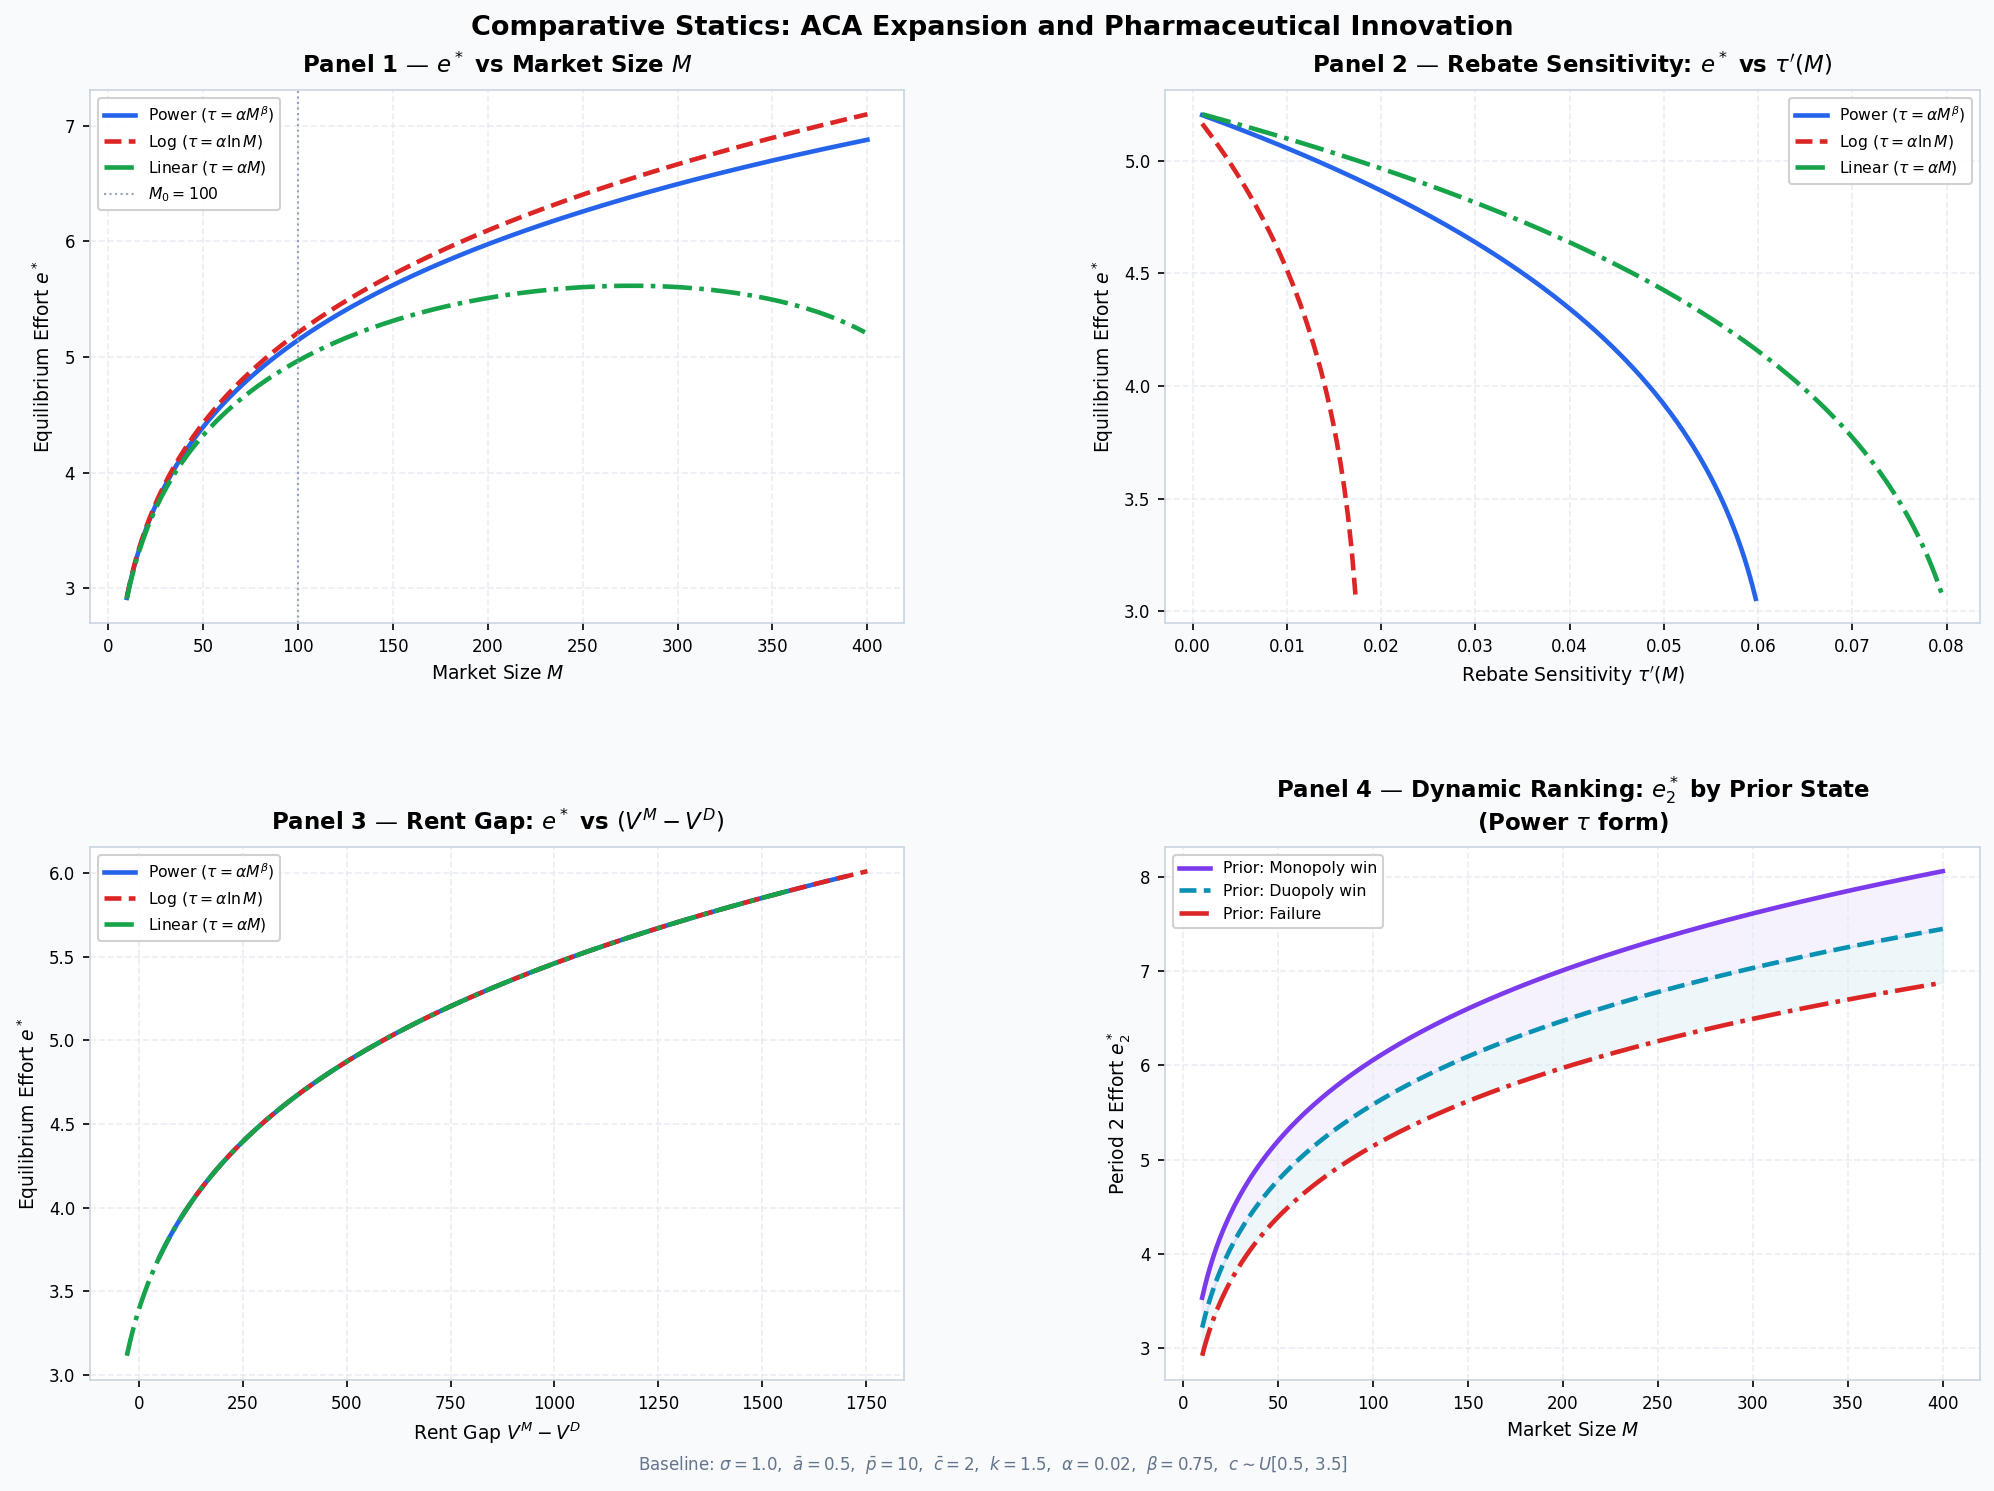
\includegraphics[width=\textwidth]{HT_week8_model.png}
    \caption{Comparative statics of equilibrium effort $e^*$. Baseline parameters: \\ $\sigma = 1.0$, $\bar{a} = 0.5$, $\bar{p} = 10$, $\bar{c} = 2$, $k = 1.5$, $\alpha = 0.02$, $\beta = 0.75$, $c \sim U[0.5, 3.5]$.}
    \label{fig:comp_statics}
\end{figure}

\paragraph{Panel 1: Equilibrium effort and market size.}
The first panel displays $e^*$ as a function of market size $M$ for each $\tau(M)$ specification. Under the logarithmic and power forms ($\beta = 0.75$), effort rises monotonically with $M$ indicating the the volume effect dominates the rebate effect, that is, the additional revenue from serving a larger market dominates, and firms invest more in R\&D as the market expands. The linear form, however, produces a hump-shaped profile. Effort initially increases with $M$ but subsequently declines, tracing out precisely the incentive trap mechanism. This shift occurs since the linear rebate schedule $\tau = \alpha M$ implies a constant marginal rebate rate, so the monopsony extraction grows one-for-one with market size. Once $M$ is large enough, the term $M\tau'(M) = \alpha M$ dominates the volume gain $(\bar{p} - \bar{c} - \tau)$, so $dV^M/dM < 0$ and the marginal benefit of effort falls.

\paragraph{Panel 2: Equilibrium effort and rebate sensitivity.}
The second panel holds $M$ fixed at the baseline value $M_0 = 100$ and varies the rebate scale parameter $\alpha$, therefore mapping the resulting $\tau'(M)$ against equilibrium effort $e^*$ and isolating the monopsony channel. Across all three $\tau$ specifications, equilibrium effort is strictly decreasing in $\tau'(M)$. Irrespective of functional form, the direction of the effect is unambiguous, and the magnitude is governed by how aggressively $\tau$ responds to market size. The result is consistent with the FOC, in which the marginal benefit of effort is proportional to $(1 - Q)V^M + QV^D$, and $V^M$ falls whenever the rebate extracted per unit of market size increases.

The curves diverge substantially in the rate of decline. The logarithmic form exhibits the steepest collapse, while the linear and power forms sustain higher efforts across a wider range of sensitivity values before $V^M$ is fully eroded. 

\paragraph{Panel 3: Equilibrium effort and the rent gap.}
The third panel varies the price cap $\bar{p}$ to trace equilibrium effort $e^*$ as a function of the rent gap $V^M - V^D$. It shows that innovation is driven by the gap between monopoly and duopoly payoffs, rather than by the level of either payoff alone. Because the first-order condition depends on this rent differential, the relationship between $e^*$ and $V^M - V^D$ is independent of the specific rebate functional form, which is why the curves overlap. Any policy that compresses the monopoly premium - through a higher rebate wedge, a lower price cap, or stronger competition in procurement — lowers equilibrium effort. The relationship is also non-linear: effort falls sharply as the rent gap approaches zero, while larger rent gaps yield smaller marginal increases in effort.

\paragraph{Panel 4: Period 2 effort by prior state.}
The fourth panel illustrates the dynamic ranking result under the power specification $\tau(M)=\alpha M^{\beta}$. For each value of $M$, period 2 equilibrium effort is computed under three cost parameters corresponding to the three possible period 1 outcomes: a monopoly win, a duopoly win, and failure. The ranking
\[
e_2^*(V^M) > e_2^*(V^D) > e_2^*(0)
\]
holds throughout. This is consistent with the model's dynamic mechanism: firms that secure higher rents in period 1 face lower effective R\&D costs in period 2 and therefore invest more in subsequent innovation. The gaps between the three paths widen with market size, showing that the long-run innovation consequences of period 1 procurement outcomes become stronger in larger markets. In this sense, current procurement outcomes do not simply affect contemporaneous profits; they also shape the future distribution of innovative effort across firms.

Taken together, the four panels provide a consistent picture of the model's predictions. The incentive trap arises once rebate growth with market size is sufficiently strong. Innovation appears to be governed by the rent gap $(V^M - V^D)$ rather than by any functional form of $\tau(M)$. The dynamic extension further shows that these effects persist over time, since weaker current rents translate into weaker future innovation incentives.



\subsection{Theoretical States and Empirical Outcomes}
To bridge the theoretical framework with the empirical PDL counterfactual analysis, the regression variables are mapped directly to the realised outcomes of the game's two-hurdle structure.  Empirically, the pharmaceutical procurement pipeline is observed through three sequential indicators: passing clinical approval, submitting a pricing bid, and ultimately gaining preferred status.  In the context of the model, these variables represent different realised ex-post paths of partial versus full success:

\begin{itemize}
    \item \textbf{Full Market Access:} These are firms that secure the Monopoly state (Stage 3a) or actually win the Duopoly auction (Stage 3b). In this scenario, they clear all hurdles and capture the market $M$. They benefit from both channels of state-dependent innovation: they accumulate regulatory know-how while also realising a strictly positive ex-post internal cash flow ($V^M$ or $V^D$). Consequently, they secure a strictly lower marginal cost of future R\&D effort ($k(V^M)$ or $k(V^D)$), allowing them to overcome market disincentives.
    
    \item \textbf{Partial Success:} These represent firms that exert sufficient effort to clear the clinical stage ($a_i \ge \bar{a}$) and enter the price stage (Stage 3b), but ultimately lose to a lower bidder in the bidding game. While clearing the clinical hurdle provides these firms with some accumulated regulatory know-how, the auction uncertainty has converged to failure. They capture zero volume and realise an ex-post payoff of zero ($\pi_{i,1} = 0$). Due to receiving no internal cash flows to alleviate capital market frictions, their cost parameter remains strictly higher than that of the PDL winners, falling in some intermediate interval $k \in (k(V^D), k(0))$. This relative cost disadcantage causes subsequent innovation to decline once combined with rebate disincentives.
\end{itemize}

The negative coefficients on the partial success stages captures the aggregate disincentive caused by the Medicaid expansion. Following the ACA expansion, states leveraged their expanded market size $M$ to extract a deeper monopsony rebates $\tau(M)$, resulting in the expected profits to collapse. Firms that reach these intermediate stages expend the cost of effort to clear the hurdles, but realise no cash flows, so their subsequent R\&D efforts decline.

Conversely, the highly positive coefficient on full market access is driven by state dependent innovation. Firms that actually gain PDL status secure the internal cash flows required to bypass capital market frictions. This influx of capital strictly lowers their future cost of effort parameter ($k$). For these winners, the reduction in the marginal cost of R\&D effort outweighs the aggregate marginal benefit compression, resulting in a net increase in subsequent innovation effort relative to their off-PDL rivals.

\subsection{Policy Implications}
The model highlights a central policy trade-off in public pharmaceutical procurement. As the Medicaid market size expands, states are able to negotiate deeper supplemental rebates and thereby reduce current expenditure. However, if these rebates compress monopoly rents too aggressively, they also weaken the returns to successful innovation and reduce firms' incentives to invest in R\&D.

This suggests that the effect of Medicaid expansion on innovation depends critically on institutional design. In the model, the mechanism does not operate through insurance coverage in itself, but through the interaction of broader coverage with procurement rules that increase monopsony power and erode post-approval profits. The relevant policy question is therefore how to contain public spending without eliminating the rents needed to sustain future innovation.

The model points to two distinct policy margins. The first operates through expected returns: procurement design determines the payoff from successful innovation through the rebate wedge $\tau(M)$. Policies that make rebates increase too steeply with market size risk substantially reducing the value of the monopoly state and thereby weakening the incentive to innovate. The second operates through the cost of innovation: firms' incentives can also be supported by lowering the effective cost of effort $k$, for example through R\&D subsidies, tax credits, or policies that reduce the cost of clinical development.

Since PDL success affects future innovation through both internal cash flows and accumulated organisational capability, policies that compress current rents may have persistent effects on future R\&D. Aggressive rebate extraction may reduce not only contemporaneous innovation effort, but also the resources and capabilities needed to support subsequent innovation. Procurement policy should therefore be assessed not only in terms of immediate fiscal savings, but also in terms of its longer-run effects on pharmaceutical innovation incentives.

More broadly, the model does not imply that the expansion of public coverage is inherently in conflict with innovation. Rather, the key issue is the design of the procurement institutions attached to that coverage. If larger Medicaid markets enable states to extract substantially deeper rebates, then the short-run savings from lower prices may come at the cost of weaker innovation incentives. Where this trade-off is especially severe, a more balanced policy approach may require either limiting the growth of the rebate wedge for highly innovative drugs or offsetting weaker post-approval returns through stronger public support for R\&D.

\newpage

\bibliographystyle{apalike}
\bibliography{references}

\end{document}